\documentclass[../ana1.tex]{subfiles}
\begin{document}
\setcounter{section}{16}
\section{Eigenschaften stetiger Funktionen}
\begin{defi}[Gleichmäßige Stetigkeit]
    Eine Funktion \( f: D \rightarrow \C \) 
    heißt gleichmäßig stetig, falls
    \[ \forall \, \varepsilon > 0 \,\exists \, 
    \delta > 0 \,\forall \, z_1, z_2 \in D \text{ mit } 
    \abs{z_1 - z_2} < \delta \Rightarrow 
    \abs{f(z_1) - f(z_2)} < \varepsilon. \]
\end{defi}
\begin{bem}
    Beachte: \( \delta \) hängt nun von \(\varepsilon \) ab.
\end{bem}
\begin{bspe}\leavevmode
    \begin{enumerate}
        \item \( f: (0,1] \rightarrow \R, 
        x \mapsto \frac{1}{x} \) ist stetig in jedem 
        \( x_0 \in (0,1]. \) \\
        Wähle \( \delta := 
        \min(\frac{x_0}{2}, \frac{x_0^2 \varepsilon}{2}) \).
        Dann gilt: \( \abs{f(x) - f(x_0)} 
        \leq \frac{ 2 \abs{x-x_0} }{ x_0^2 } < \varepsilon \).\\
        Man sieht, dass das benutzte \( \delta \) umso
        kleiner wird, je mehr man sich dem linken Rand
        von \( (0,1] \) annähert.\\
        \begin{center}
            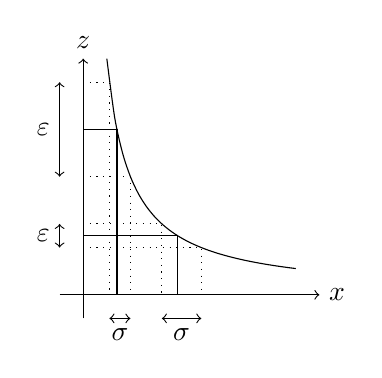
\begin{tikzpicture}[scale = 3]
                \draw[->] (0,-0.1) -- (0,1) node[above] {\(z\)};
                \draw[->] (-0.1,0) -- (1,0) node[right] {\(x\)};
                \draw[thin,domain=0.1:0.9,smooth,variable=\x,black] plot ({\x},{1 / (10 * \x)});
                \draw[dotted] (0,0.9) -- (0.111,0.9) -- (0.111,0);
                \draw[dotted] (0,0.5) -- (0.2,0.5) -- (0.2,0);
                \draw (0,0.7) -- (0.1429,0.7) -- (0.1429,0);
                \draw[<->] (-0.1,0.5) -- (-0.1,0.9) node[midway, left] {\( \varepsilon \)};
                \draw[<->] (0.111,-0.1) -- (0.2,-0.1) node[midway, below] {\(\sigma \)};

                \draw[dotted] (0,0.3) -- (0.333,0.3) -- (0.333,0);
                \draw[dotted] (0,0.2) -- (0.5,0.2) -- (0.5,0);
                \draw (0,0.25) -- (0.4,0.25) -- (0.4,0);
                \draw[<->] (-0.1,0.2) -- (-0.1,0.3) node[midway, left] {\( \varepsilon \)};
                \draw[<->] (0.333,-0.1) -- (0.5,-0.1) node[midway, below] {\(\sigma \)};

            \end{tikzpicture}
        \end{center}
        \( f \) ist nicht gleichmäßig stetig in \( (0,1] \),
        da man \( \delta \) nicht unabhängig von \(x\) wählen
        kann.\\
        Wäre \( f \) gleichmäßig stetig, so könnte man zu 
        \( \varepsilon = 1 \) ein \( \delta > 0 \) wählen,
        sodass \( \abs{ f(x) - f(\tilde{x}) } < 1 
        \,\forall \, x, \tilde{x} \in (0,1] \) mit 
        \( \abs{ x - \tilde{x} } < \delta (*) \).\\
        Es gibt aber ein \( n \geq 1 \) mit 
        \( \abs{ \frac{1}{n} - \frac{1}{2n} } < \delta \)
        und \( \abs{ f(\frac{1}{n}) - f(\frac{1}{2n}) } 
        = n \geq 1 \).
        \item Jede gleichmäßig stetige Funktion ist stetig.
        \item \( f: \R \rightarrow \R, x\mapsto x^2 \) ist stetig,
        aber nicht gleichmäßig stetig. 
        Aber \( g: [-1, 1] \rightarrow \R, x \mapsto x^2 \)
        ist gleichmäßig stetig.
    \end{enumerate}
\end{bspe}
\begin{satz}[Satz von Heine]
    Sei \( D \subset \C \) abgeschlossen und beschränkt
    und \( f: D \rightarrow \C \) stetig.\\
    Dann ist \(f\) gleichmäßig stetig.
\end{satz}
\begin{bew}
    Angenommen \(D\) ist abgeschlossen und beschränkt und
    \( f: D \rightarrow \C \) ist stetig, aber nicht gleichmäßig
    stetig (\( \leadsto \) Widerspruch)\\
    \( f \) nicht gleichmäßig stetig heißt:
    \[ \exists \, \varepsilon > 0 \,\forall \, 
    \delta > 0 \,\exists \, u, w \in D: \abs{u-w}
    < \delta \text{ und } \abs{f(u) - f(w)} \geq \varepsilon \]
    Wähle \( n\in\N, \delta = \frac{1}{n} \). Das heißt, 
    es gibt \( {(x_n)}_n, {(y_n)}_n \subseteq D \) mit 
    \( \abs{x_n - y_n} < \frac{1}{n} \) und 
    \( \abs{f(x_n) - f(y_n)} \geq \varepsilon \) für 
    \( n\in\N \).\\
    Da \( {(y_n)}_n \subseteq D \) und \( D \) beschränkt ist,
    existiert eine konvergente Teilfolge von \( {(y_n)}_n \).
    \( \exists \, \sigma : \N \rightarrow \N,
    \sigma(n) < \sigma(n+1) \,\forall \, n\in\N \), 
    sodass \( y_{\sigma(k)} \) konvergiert.\\
    \( z_0 := \limes{k} y_{\sigma(k)} \). Da \(D\) abgeschlossen
    ist und \( y_{\sigma(k)} \in D \,\forall \, k \in\N \), 
    ist \( z_0 \in D \).\\
    Betrachte Teilfolge \( \tilde{x}_k := x_{\sigma(k)} \).
    Dann gilt:
    \[ \abs{ \tilde{x}_k - y_{\sigma(k)} } 
    = \abs{ x_{\sigma(k)} - y_{\sigma(k)} }
    < \frac{1}{\sigma(k)} \rightarrow 0. \]
    Da \( y_{\sigma(k)} \rightarrow z_0 \), folgt 
    \( \abs{ \tilde{x}_k - z_0 } \rightarrow 0. \) \\
    Also \( \limes{k} \tilde{x}_k = z_0 \) und 
    \begin{align*}
        \varepsilon \leq &\abs{ f(x_{\sigma(k)}) - f(y_{\sigma(k)}) }\\
        = &\abs{ f(x_{\sigma(k)}) - f(z_0) + f(z_0) - f(y_{\sigma(k)}) }\\
        \leq &\abs{ f(x_{\sigma(k)}) - f(z_0) } + \underbrace{\abs{ f(z_0) - f(y_{\sigma(k)}) }}_{\longrightarrow 0}
    \end{align*}
    Es ist also 
    \[ \limesinf{k} \abs{ f(x_{\sigma(k)}) - f(z_0) } \geq \varepsilon > 0 \text{ \Lightning{} zu Stetigkeit von  } f \text{ in } x_0. \]
\end{bew}
\end{document}